%%%%%%%%%%%%%%%%%%%%%%%%%%%%%%%%%%%%%%%%%
% Journal Article
% LaTeX Template
% Version 1.3 (9/9/13)
%
% This template has been downloaded from:
% http://www.LaTeXTemplates.com
%
% Original author:
% Frits Wenneker (http://www.howtotex.com)
%
% License:
% CC BY-NC-SA 3.0 (http://creativecommons.org/licenses/by-nc-sa/3.0/)
%
%%%%%%%%%%%%%%%%%%%%%%%%%%%%%%%%%%%%%%%%%

%----------------------------------------------------------------------------------------
%	PACKAGES AND OTHER DOCUMENT CONFIGURATIONS
%----------------------------------------------------------------------------------------

\documentclass[twoside]{article}
\usepackage{lipsum} % Package to generate dummy text throughout this template
\usepackage[superscript]{cite}
\usepackage[sc]{mathpazo} % Use the Palatino font
\usepackage[T1]{fontenc} % Use 8-bit encoding that has 256 glyphs
\linespread{1.05} % Line spacing - Palatino needs more space between lines
\usepackage{microtype} % Slightly tweak font spacing for aesthetics
\usepackage{amsthm}
\usepackage[margin=0.5in, top=30mm,columnsep=50pt]{geometry} % Document margins
\usepackage{multicol} % Used for the two-column layout of the document
\usepackage[hang, small,labelfont=bf,up,textfont=it,up]{caption} % Custom captions under/above floats in tables or figures
\usepackage{booktabs} % Horizontal rules in tables
\usepackage{float} % Required for tables and figures in the multi-column environment - they need to be placed in specific locations with the [H] (e.g. \begin{table}[H])
\usepackage{hyperref} % For hyperlinks in the PDF
\usepackage{graphicx}
\usepackage{lettrine} % The lettrine is the first enlarged letter at the beginning of the text
\usepackage{paralist} % Used for the compactitem environment which makes bullet points with less space between them
\usepackage{ulem}
\usepackage{empheq}
\newcommand*\widefbox[1]{\fbox{\hspace{2em}#1\hspace{2em}}}
\usepackage{amsmath}
\usepackage{amsfonts}
\newtheorem*{hyp*}{Hypothesis}

\usepackage{abstract} % Allows abstract customization
\renewcommand{\abstractnamefont}{\normalfont\bfseries} % Set the "Abstract" text to bold
\renewcommand{\abstracttextfont}{\normalfont\small\itshape} % Set the abstract itself to small italic text

\usepackage{titlesec} % Allows customization of titles
\renewcommand\thesection{\Roman{section}} % Roman numerals for the sections
\renewcommand\thesubsection{\Roman{subsection}} % Roman numerals for subsections
\titleformat{\section}[block]{\large\scshape\centering}{\thesection.}{1em}{} % Change the look of the section titles
\titleformat{\subsection}[block]{\large}{\thesubsection.}{1em}{} % Change the look of the section titles

\usepackage{fancyhdr} % Headers and footers
\pagestyle{fancy} % All pages have headers and footers
\fancyhead{} % Blank out the default header
\fancyfoot{} % Blank out the default footer
\fancyhead[C]{Imperial College London$\bullet$ March 2014 $\bullet$ Henry O'Hagan } % Custom header text
\fancyfoot[RO,LE]{\thepage} % Custom footer text
\usepackage{perpage} %the perpage package
\MakePerPage{footnote} %the perpage package command



\usepackage{mathtools}
\DeclarePairedDelimiter\ceil{\lceil}{\rceil}
\DeclarePairedDelimiter\floor{\lfloor}{\rfloor}

%----------------------------------------------------------------------------------------
%	TITLE SECTION
%----------------------------------------------------------------------------------------

\title{\vspace{-15mm}\fontsize{18pt}{10pt}\selectfont\textbf{Scale-Free Stochastic Networks}\vspace{-15mm}} % Article title

\date{}

%----------------------------------------------------------------------------------------

\begin{document}
\normalem
\maketitle % Insert title

\thispagestyle{fancy} % All pages have headers and footers

%----------------------------------------------------------------------------------------
%	ABSTRACT
%----------------------------------------------------------------------------------------

\begin{abstract}

\noindent 
This report will look into the underlying mechanisms of fat tailed degree distributions in real-world networks. A proposed underlying mechanism for this phenomenon is preferential attachment, which is in practice implemented via the Barabasi-Albert model of a growing network. After analysis on the degree distributions of the Barabasi-Albert model, this will be compared to other schemes, using random attachment and random walks. The results show that the fat tailed distributions occur in the Barabasi-Albert model, and also using random walks, for the length of the walk $L>1$. The random attachment model exhibits an exponential cut-off. Performing a chi-square test for both the Barabasi-Albert model and the random attachment model, comparing the data to the theoretical forms, the resulting p-values gave no reason to doubt the theoretical derivations. For the Barabasi-Albert model, the predicted largest value of the degree did not match the mean average of the largest observed degree, but it matched the modal average, it was hypothesised that this effect could be due to the high skewness and kurtosis in fat-tailed distributions. The random walks appeared to follow fat tailed distributions for $L>1$, but had an even higher skewness and kurtosis for $L=1$. The $L=0$ case appeared to follow the same form of the random attachment distribution.
\end{abstract}

%----------------------------------------------------------------------------------------
%	ARTICLE CONTENTS
%----------------------------------------------------------------------------------------

{\let\thefootnote\relax\footnote{Word Count:2400}}

\vspace{-5mm}
\section{Aims \& Introduction}

\lettrine[nindent=0em,lines=2]{T}he Barabasi-Albert, or price model is a network model that uses the concept of preferential attachment. This more closely resembles the citation network (where the degree is the number of citations and the nodes are scientific papers) than the Erdos-Reyni random graphs. Citation networks, have a fat-tailed distribution, so that the degrees are present on all scales. The aims are to investigate the Barabasi-Albert model, in terms of how well theoretical predictions match with the simulated degree distribution, this will also be done for random attachment. Then the report will look into using random walks on the network as the mechanism for choosing which edges are connected.

%------------------------------------------------METHOD

\section{Methods}
\subsection{Algorithm}
The algorithm used is defined as follows:\cite{script}
\begin{enumerate}
\item Set up initial network $\mathcal{G}_0$ 
\item Increment time $t \to t +1 $
\item Add one new node
\item Add $m$ edges as follows:
\begin{itemize}
\item Connect one end of the new edge to the new node.
\item Connect the other end to an existing node with probability $\Pi$
\end{itemize}
\item Repeat from 2
\end{enumerate}
In the script that was written, there was no need to increment time, since it is proportional to the number of nodes and the number of nodes is automatically known by the ``graph'' object, creating a time variable and incrementing it would have caused a slight inefficiency. The initial network that was used was a complete network with the number of nodes equal to $m+1$, this was so that all the initial nodes had the minimum degree $k=m$. For preferential attachment (Barabasi-Albert model) $\Pi \propto k$, for random attachment $\Pi \propto \text{constant}$.

In the case of using random walks in order to choose the nodes that are connected to the new node, after setting up an initial network, choose a node at random, and pick any neighbouring node from the currently selected node at random, do this $L$ times, the last node to be selected is then the vertex to be added. This process is then repeated $m$ times. The program was checked to be working by querying the graphs for node number and degree at each time step, and seeing that the node number increases by 1 at each time step and edge number increasing by $m$ at each time step. The parameters required by the program are $m$, and the method for which to choose which vertices to connect to.

\subsection{Derivation of Degree Distribution for Preferential Attachment}
The master equation for the Barabasi-Albert model is
\[
n(k,t+1) = n(k,t) +m\Pi (k-1,t) n(k-1 , t) - m \Pi (k,t) n (k,t) +\delta_{km}
\]
where $n$ is the number of nodes of degree $n$. The first term on the right $n(k,t)$ comes from the starting number at time $t$, the second term $m\Pi (k-1,t) n(k-1 , t)$ comes from the average number of nodes with degree $k-1$ that is increased in degree as a result of one time step. The third term $m \Pi (k,t) n (k,t)$ comes from the average number of nodes with degree $k$ that is increased in degree as a result of a time step. The $\delta_{km}$ term comes from the node that is added with degree $m$. 

The probability $\Pi$ is given by:
\[
\Pi(k,t) = \frac{k}{2E(t)} = \frac{k}{2mN(t)}
\]
where $E$ is the number of edges at time $t$, since the number of edges added is $m$ each time, it's proportional to the number of nodes $N$ with proportionality constant $m$. In terms of probability distribution $p(k,t) = n(k,t)/N(t)$:
\[
N(t+1)p(k,t+1) - N(t) p(k,t) = \frac{1}{2} \left[ (k-1) p(k-1,t) - k p(k,t) \right] + \delta_{km}
\]
Since $N(t+1) = 1+N(t)$, taking the limit as $t \to \infty$ of $p$, $p(k,t) \to p_{\infty} (k)$:
\[
p_{\infty}(k) = \frac{1}{2} \left[(k-1) p_{\infty} (k-1) - k o_{\infty}(k) \right] +\delta_{km}
\]
First assuming that $k \neq m$ rearranging this gives:
\[
\frac{p_{\infty}(k) }{p_{\infty}(k-1)} = \frac{k-1}{k+2}
\]
which has the solution,
\[
p_{\infty}(k)=A\frac{\Gamma (k)}{\Gamma (k+3) } = \frac{A}{k(k+1)(k+2)}
\]
for any $A$. Considering the case where $m=k$ and $p_{\infty} (m-1) =0$, gives,
\begin{align*}
p_{\infty}(m) & = 1 - \frac{m p_{\infty}(m)}{2} \\
\implies p_{\infty}(m) & = \frac{2}{m+2}
\end{align*}
This gives the normalisation constant $A$:
\begin{align*}
\frac{A}{(m+2)(m+1)m} & \overset{!}{=} \frac{2}{m+2} \\
\implies A &= 2m(m+1)
\end{align*}
Thus:
\[
\boxed{
p_{\infty} (k) = \frac{2m(m+1)}{k(k+1)(k+2)} \quad \text{for } k \geq m}
\]
Checking whether this is normalised:
\begin{align*}
\sum_{k=m}^{\infty}p_{\infty}(k)&= \sum_{k=m}^{\infty}  \frac{2m(m+1)}{k(k+1)(k+2)} \\
&= \sum_{k=m}^{\infty} \frac{m(m+1)}{k} - \frac{2m(m+1)}{k+1} +\frac{m(m+1)}{k+2} \\
&= (m+1) - 2m + \frac{m(m+1)}{m+2}\\
&+ \; m \;  - \frac{2m(m+1)}{m+2} + \;\;\; \vdots \\
&+  \frac{m(m+1)}{m+2} - \vdots\;\;\; + \;\;\; \vdots \\
&= 1
\end{align*}
As required.
\subsection{Derivations of Degree Distribution for Random Attachment}
The form of the master equation is unchanged, this time the attachment probability is:
\[
\Pi (k,t) = \frac{1}{N(t)} = \frac{1}{t+N(0)}
\]
substituting into the master equation gives:
\[
n(k,t+1) - n(k,t) = \frac{m}{t+t_0} (n(k-1, t) - n(k,t) ) + \delta_{km}
\]
substituting $p(k,t)=n(k,t)/N(t)$:
\[
(t+1+N(0)) p(k,t+1) - (t+N(0)) p(k, t) = m ( p(k-1, t) - p(k,t) ) +\delta_{km}
\]
Taking $t \to \infty$:
\begin{equation}
p_{\infty}(k)=m ( p_{\infty}(k-1)- p_{\infty}(k)) +\delta_{mn}
\end{equation}
Starting from this equation there are two methods that is used to derive $p_{\infty}$(k).
\subsubsection{Method I}
Assume $k \neq m$, then rearrange equation 1:
\[
p_{\infty} (k) =mp_{\infty} (k-1) / (m+1)
\]
for the $k=m$ case:
\[
p_{\infty} (m)= \delta_{mm}/(m+1)=1/(m+1)
\]
Setting $p_{\infty} (m-1)=0$ as before. Hence, iterating the previous equation we can conclude that:
\[
\boxed{
p_{\infty}(k) =\frac{1}{m+1} \left( \frac{m}{m+1} \right)^{k-m}  \quad \text{for } k \geq m}
\]
Checking the normalisation:
\begin{align*}
\sum_{k=m}^{\infty} p_{\infty} (k) &= \frac{1}{1+m} \sum_{k=m}^{\infty} \left( \frac{m}{m+1} \right)^{k-m} \\
&=  \frac{1}{1+m}  \sum_{k=0}^{\infty} \left( \frac{m}{m+1} \right)^{k} \\
&= \frac{1}{(1+m)} \frac{1}{(1-\frac{m}{m+1})} \\
&= 1
\end{align*}
As required.
\subsubsection{Method II}

The probabilities can be transformed using a discrete mellin transform:\cite{cc}
\[
G_{\infty} (k) = \sum_k^{\infty} z^k p_{\infty} (k)
\]
Multiplying equation 1 by $z^k$ and summing over all $k$ gives:
\begin{align*}
G_{\infty} (k) &= z^m -mG_{\infty} (k) + \sum_{k} m z^k p_{\infty}(k-1) \\
G_{\infty} (k)(1+m) &= z^m+ \sum_k z^{k+1} p_{\infty} (k) \\
G_{\infty} (k)(1+m) &= z^m + mz G_{\infty} (k)\\
G_{\infty}(k) & = \frac{z^m/m}{\frac{1+m}{m}-z}
\end{align*}
Now using the inverse Mellin transform, the probabilities are obtained:
\begin{align*}
p_{\infty} (k) &= \mathcal{M}^{-1} [G_{\infty}(z)] = \frac{1}{2\pi i} \int_{c-i\infty}^{c+i\infty} z^{-k-1} G_{\infty}(z)\, \mathrm{d} z \\
p_{\infty} (k) &=  \frac{1}{2m\pi i} \int_{c-i\infty}^{c+i\infty}  \frac{z^{m-k-1}}{\frac{1+m}{m}-z} \mathrm{d} z 
\end{align*}
Where $c \in [0,\frac{1+m}{m}]$ (in this particular case), is between the regions on the complex plane in which there are residues in the integrand.

Consider:
\[
\frac{\mathrm{Res}(f(z),z_0)}{m}=\frac{1}{2m\pi i} \lim_{R \to \infty} \left( \int_{c-iR}^{c+iR}  \frac{z^{m-k-1}}{\frac{1+m}{m}-z} \mathrm{d} z  +  \int_{\mathcal{C}\in \mathbb{C}}  \frac{z^{m-k-1}}{\frac{1+m}{m}-z} \mathrm{d} z  \right)
\]
where $\mathcal{C}$ encloses a semicircle from $-iR$ to $iR$, in either direction/chirality, $f(z)$ is the integrand $\frac{z^{m-k-1}}{\frac{1+m}{m}-z} $, and $z_0$ is the location of either of its residues.

Using the substitution $z=R e^{i\theta} -c$, $\mathrm{d} z = iz \mathrm{d} \theta$
\begin{align*}
\left| \int_{\mathcal{C}\in \mathbb{C}}  \frac{z^{m-k}}{\frac{1+m}{m}-z}i \mathrm{d} \theta \right| &<  \int_{\mathcal{C}\in \mathbb{C}} \left| \frac{z^{m-k}}{\frac{1+m}{m}-z} \right| \mathrm{d} \theta \\
& \approx \int_{\mathcal{C}\in \mathbb{C}} \left| R^{m-k-1} \right| \mathrm{d} \theta 
\end{align*}
Which goes to zero as $R \to \infty$ for the constraint on the network $k \geq m $. Hence the integral $f(z)$ in the region $\mathfrak{Re}(z)>c$ or $\mathfrak{Re}(z)<c$ is entirely due to the vertical line in the complex plane.
\[
p_{\infty} (k)=\frac{\mathrm{Res}(f(z),z_0)}{m}
\]
Taking the Laurent expansion of $f(z)$ about $z=0$ gives, for $b:=m-k$, $a:=\frac{1+m}{m}$
\[
f(z)= z^b \left( \frac{1}{az} + \frac{1}{a^2} + \frac{z}{a^3} + \cdots \right)
\]
Taking the positive residues since on the region $\mathfrak{Re}(z)<c$ , the integral goes around the residue in a right handed chirality:
\[
\boxed{
p_{\infty} (k) = \frac{1}{m} a^{b-1} = \frac{1}{m} \left( \frac{1+m}{m} \right)^{m-k-1} = \frac{1}{m+1}  \left( \frac{1+m}{m} \right)^{m-k}}
\]
Now checking the solution, by integrating over  $\mathfrak{Re}(z)>c$, the Laurent expansion about $z=a$ is:
\[
-\frac{a^{b-1}}{z-a} - (b-1) a^{b-2} - \cdots
\]
This time taking the negative of the residue since the integral goes round the residue in a left handed chirality,
\[
p_{\infty}(k) = \frac{1}{m} a^{b-1}
\]
as before. Both methods give the same solution.

\subsection{Largest Expected Degree for a Given Network Size}
\subsubsection{Preferential Attachment Case}
network of size $N$ for large $N$ can be approximated with $p_{\infty}(k)$. For at least $1$ to have the degree $k_{max}$, the probability,
\[
P(k>k_{max}) \overset{!}{=} \frac{1}{N}
\]
Hence
\begin{align*}
1/N &= \sum_{k=k_{\text{max}}}^{\infty} \frac{2m(m+1)}{k(k+1)(k+2)} \\
&\approx m(m+1) \int_{k=k_{\text{max}}}^{\infty}  \frac{1}{k} - \frac{2}{k+1} +\frac{1}{k+2} \\
&= m(m+1) \left. \ln \left( \frac{k(k+2)}{(k+1)^2} \right) \right|_{k=k_{\text{max}}}^{\infty} 
\end{align*}
Assessing the convergence of the top limit:
\[
\lim_{k \to \infty} \ln \left( \frac{k(k+2)}{(k+1)^2} \right) = \ln (1) =0
\]
Hence,
\begin{align*}
\frac{k_{1}(k_{1}+2)}{(k_1+1)^2} &= \exp \left( \frac{-1}{Nm(m+1)} \right) \\
\implies (1- A)k_1^2 +2(1-A) k_1 - A&= 0 \\
\implies k_1 &= -1 + \sqrt{1+\frac{A}{1-A}}
\end{align*}
where $A:= \exp \left( \frac{-1}{Nm(m+1)} \right)<1$ since the argument in the exponential is always negative.

\subsubsection{Random Attachment Case}

Again use the requirement that 
\[
P(k>k_{max}) \overset{!}{=} \frac{1}{N}
\]
So that
\begin{align*}
1/N&= \sum_{k=k_1}^{\infty} p_{\infty} (k)\\
&= \frac{1}{m+1} \sum_{k=k_1}^{\infty} \left( \frac{1+m}{m} \right)^{m-k} \\
&= \left( \frac{1+m}{m} \right)^{m-k_1} \frac{1}{m+1} \sum_{k=0}^{\infty} \left( \frac{1+m}{m} \right)^{-k}\\
&= \left( \frac{1+m}{m} \right)^{m-k_1}\\
\implies k_1 &= \frac{\ln \left( N \left( \frac{m+1}{m} \right)^m \right)}{\ln \frac{m+1}{m}}
\end{align*}

%------------------------------------------------RESULTS

\section{Results}
\subsection{Preferential Attachment Case}
\subsubsection{Degree Distribution}

\begin{center}
  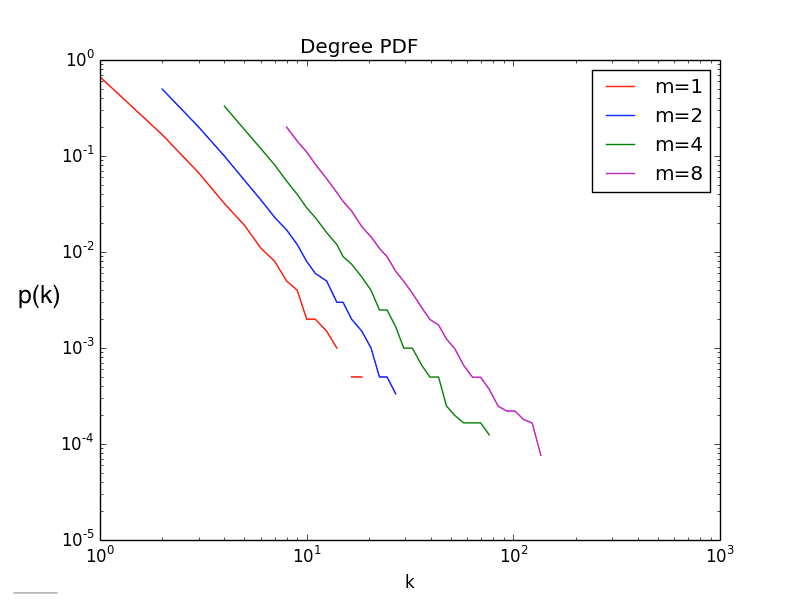
\includegraphics[height=100mm]{degree_dist.png}
  \captionof{figure}{Degree distribution for preferential attachment, for different values of $m$, log-binned to reduce the bad statistics caused by the fat tail.}\footnote{see appendix}
\end{center}
The results were obtained choosing the parameters, $m=1,2,4,8$, so that the program samples a reasonable scale in $m$, whilst not taking too long.
\begin{multicols}{2}
\begin{center}
  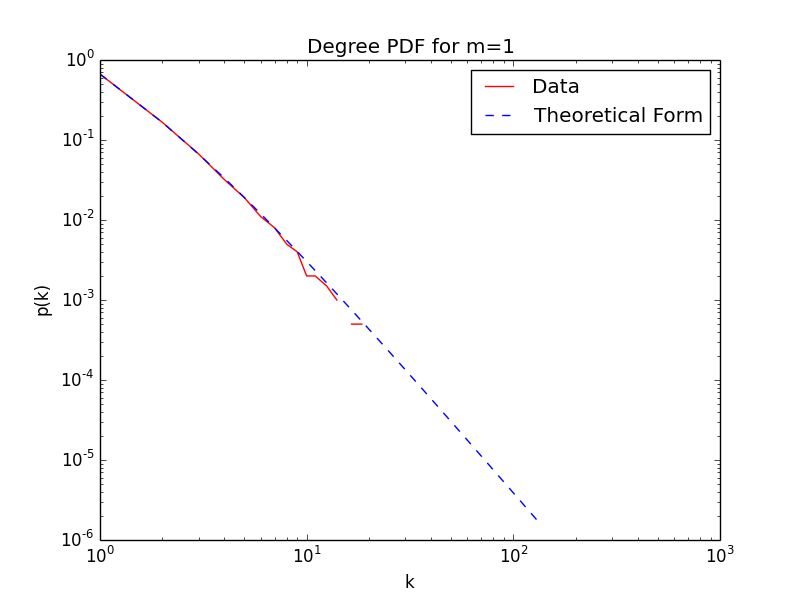
\includegraphics[height=60mm]{comparison0.png}
  \captionof{figure}{Degree distribution for preferential attachment, with theoretical values also plotted for $m=1$, log-binned to reduce the bad statistics caused by the fat tail.}
\end{center}
\begin{center}
  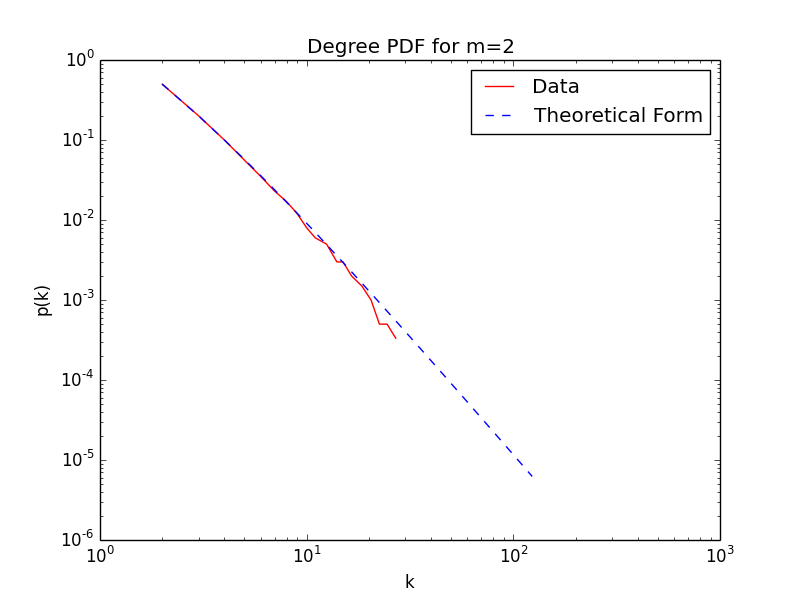
\includegraphics[height=60mm]{comparison1.png}
  \captionof{figure}{Degree distribution for preferential attachment, with theoretical values also plotted for $m=2$, log-binned to reduce the bad statistics caused by the fat tail.}
\end{center}
\begin{center}
  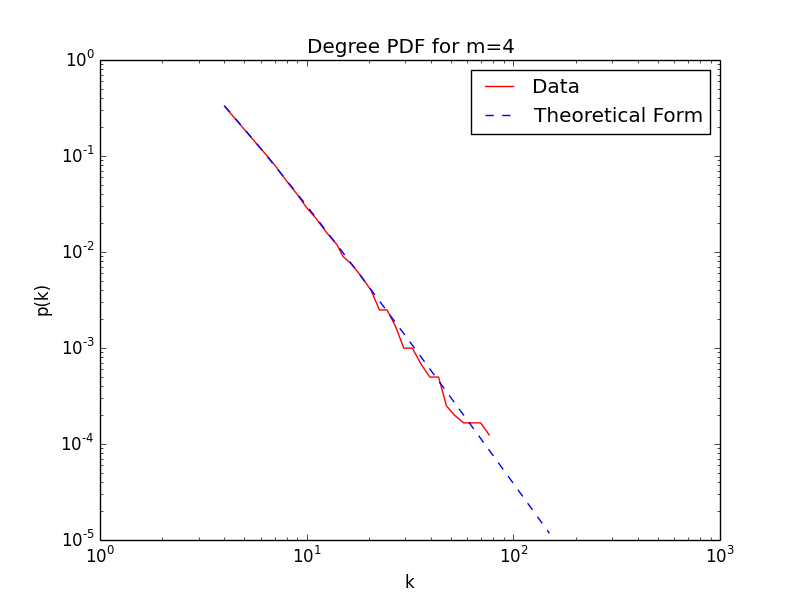
\includegraphics[height=60mm]{comparison2.png}
  \captionof{figure}{Degree distribution for preferential attachment, with theoretical values also plotted for $m=4$, log-binned to reduce the bad statistics caused by the fat tail.}
\end{center}
\begin{center}
  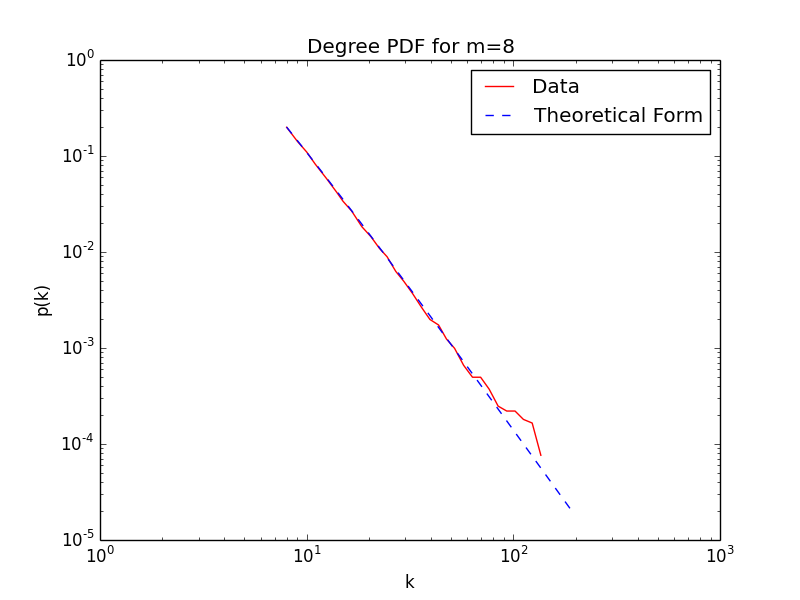
\includegraphics[height=60mm]{comparison3.png}
  \captionof{figure}{Degree distribution for preferential attachment, with theoretical values also plotted for $m=8$, log-binned to reduce the bad statistics caused by the fat tail.}
\end{center}
\end{multicols}
Compared to the theoretical result, the data matches, with some fluctuations at the tail end of the distribution. This shows that there is indeed no typical scale for the degree. A $\chi^2$-test was performed and it was found that all the p-values were 1.0 up to the accuracy of the variable type, hence there is no reasonable doubt that the theoretical model matches the simulation.
\begin{center}
    \begin{tabular}{|l|l|l|l|}
    \hline
    $m$ & $\chi^2$ & Degrees of Freedom &p-value \\ \hline
    1 & $3.40391064383 $ & $35$ & 1.0\\ \hline
    2 & $2.30599926631 $ & $34$& 1.0\\ \hline
    4 &  $0.8779577978 $ & $34$&1.0\\ \hline
    8 &  $0.757281441045$ & $33$&1.0\\ \hline
    \end{tabular}
\end{center}
\subsubsection{Finite-Size effects}
Looking at the distribution for varying numbers of nodes, it's found that the mean-averages of the maximum degree do not correspond to the theoretical values, however, the modal-average is close to the predicted values:
\begin{center}
    \begin{tabular}{|   l|  l|   l|   l|   l|   l|}
    \hline
    $N$ & $\mu(\hat{k}_l)$ &$\sigma(\hat{k}_l)$ & mode & median & predicted value \\ \hline
    101 & $19.1174 $&0.000484533360565 & $16$ & 18&13.23 \\ \hline
    1001 & $63.28 $ &0.0168545389732& $43$& 59 & 43.75\\ \hline
    10001 &  $221.9 $ &4.94349066956& $144$&190 & 140.43\\ \hline
    \end{tabular}
\end{center}
The differences between the predicted values and the observed values could be due to the high kurtosis and skewness of fat-tailed distributions, as exhibited by the data. There is no typical scale for degree distribution in the limit that the network size goes to infinity.

\begin{multicols}{2}
\begin{center}
  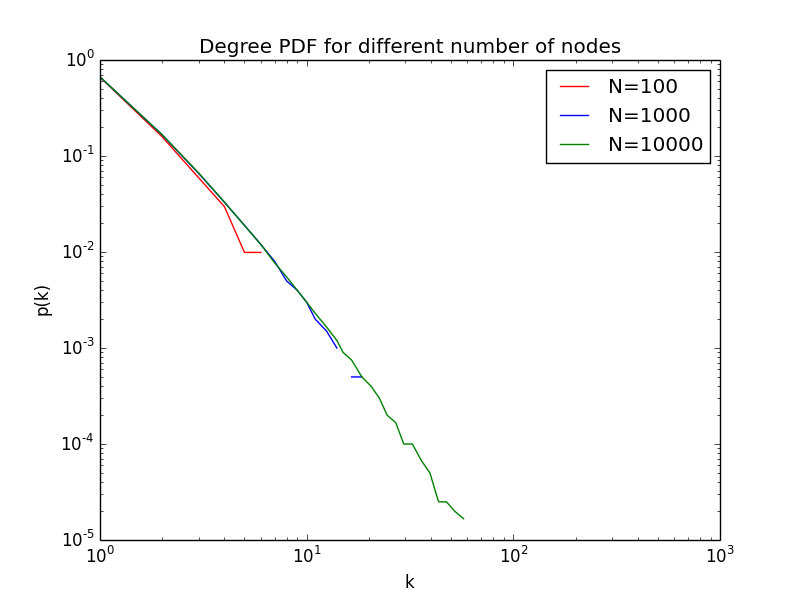
\includegraphics[height=60mm]{degree_dist_varying_N.png}
  \captionof{figure}{Degree distribution for different values of $N$, for $m=1$ log-binned to reduce the bad statistics caused by the fat tail. Averaged over multiple iterations.}
\end{center}
\begin{center}
  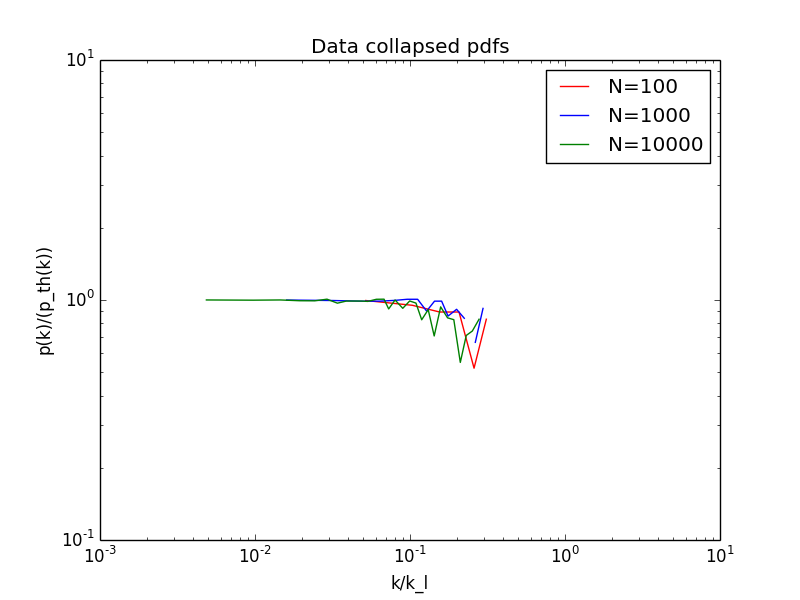
\includegraphics[height=60mm]{degree_dist_collapsed.png}
  \captionof{figure}{Collapsed degree distributions, for $m=1$}
\end{center}
\end{multicols}
The degree distributions can be collapsed by plotting $p_{data}/p_{theoretical}$ vs $k/k_1$, since the tail cut off of the distribution scales by the largest value.


\begin{multicols}{2}
\begin{center}
  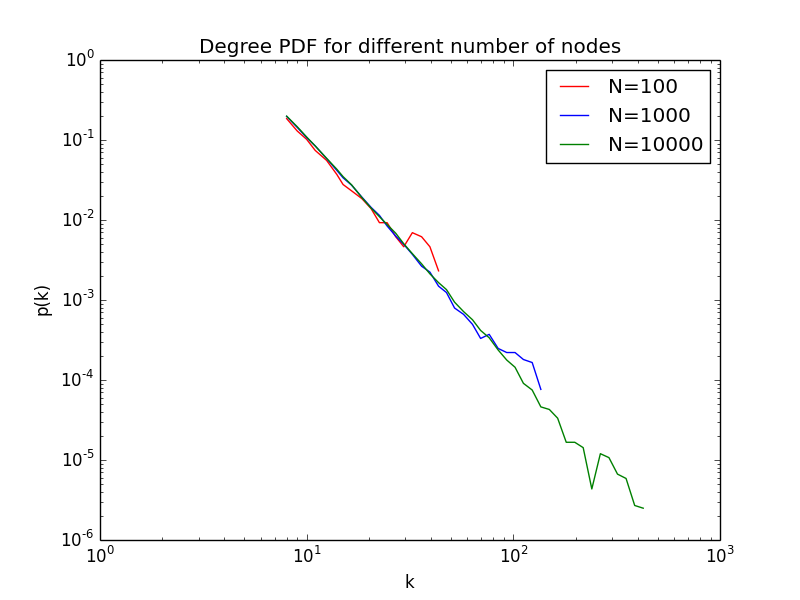
\includegraphics[height=60mm]{degree_dist_varying_N2.png}
  \captionof{figure}{Degree distribution for different values of $N$, for $m=8$ log-binned to reduce the bad statistics caused by the fat tail. Averaged over multiple iterations.}
\end{center}
\begin{center}
  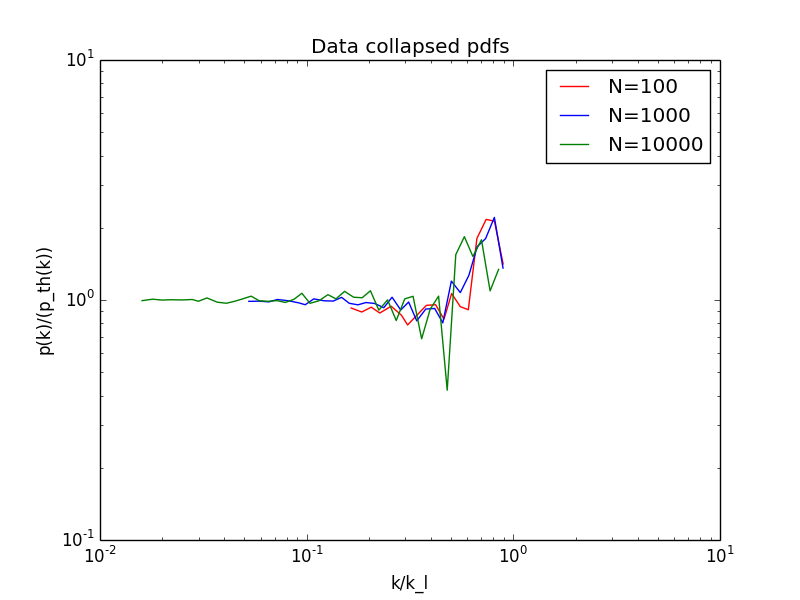
\includegraphics[height=60mm]{degree_dist_collapsed2.png}
  \captionof{figure}{Collapsed degree distributions, for $m=8$}
\end{center}
\end{multicols}
For larger values of $m$, it becomes apparent that the distribution rises for the the tail ends of the data. This occurs with all 3 profiles and thus it cannot simply be ignored and explained due to the poor statistics at the end of the fat-tailed distributions.These are caused by nodes which would otherwise have had a larger degree, if the system size was not limited. This effect is only noticeable if the network is growing fast enough, so for $m=8$ the effect is visible. On the profile of the collapsed pdf for $m=8$, all the bumps are increasing by the same order of magnitude with respect to the scaling behaviour of the largest degree, and the magnitude of the probability.

\subsection{Random Attachment Case}
\subsubsection{Degree Distribution}
\begin{center}
  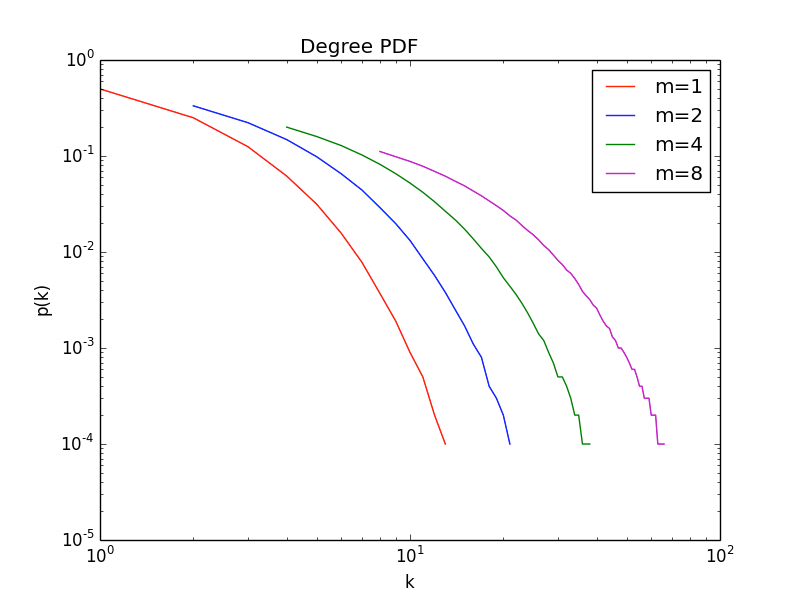
\includegraphics[height=80mm]{degree_dist_PRA.png}
  \captionof{figure}{Degree distribution for random attachment, for different values of $m$, log-binned to reduce the bad statistics caused by the fat tail.}\footnote{see appendix}
\end{center}
\begin{multicols}{2}
\begin{center}
  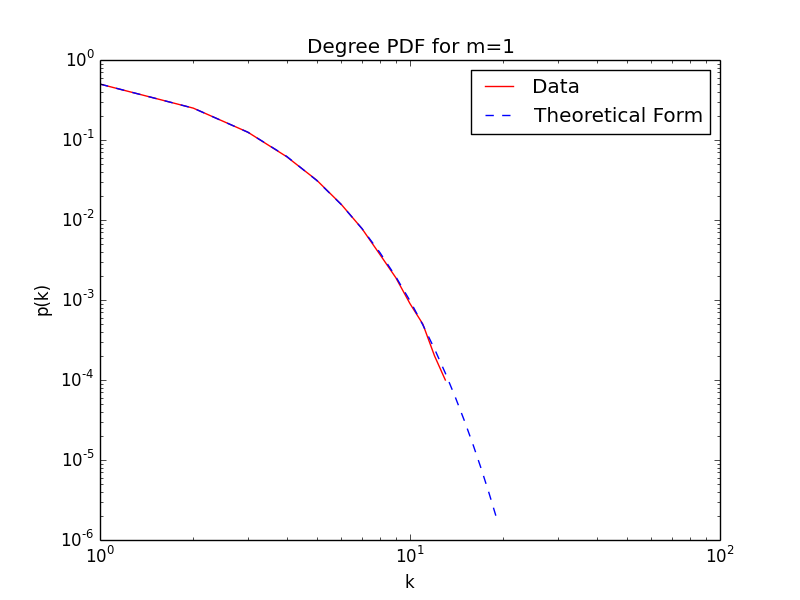
\includegraphics[height=60mm]{comparison02.png}
  \captionof{figure}{Degree distribution for random attachment, with theoretical values also plotted for $m=1$, log-binned to reduce the bad statistics caused by the fat tail.}
\end{center}
\begin{center}
  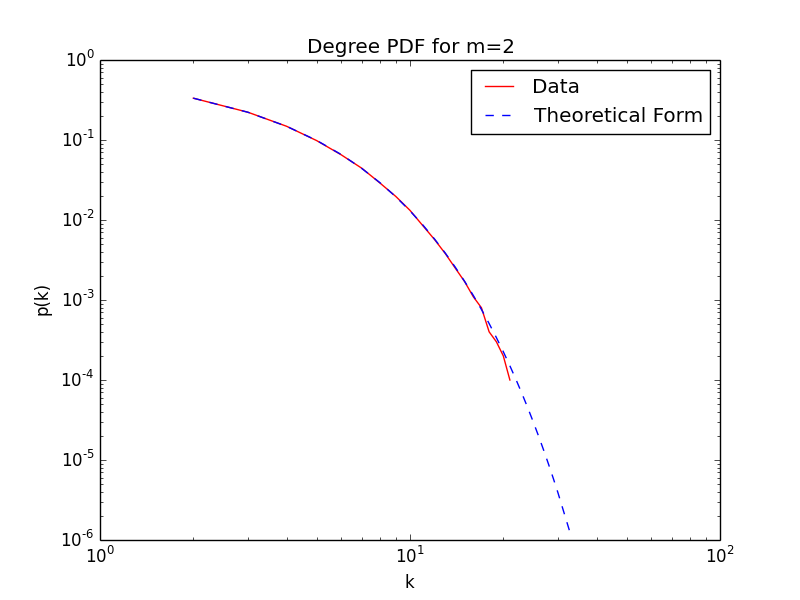
\includegraphics[height=60mm]{comparison12.png}
  \captionof{figure}{Degree distribution for random attachment, with theoretical values also plotted for $m=2$, log-binned to reduce the bad statistics caused by the fat tail.}
\end{center}
\begin{center}
  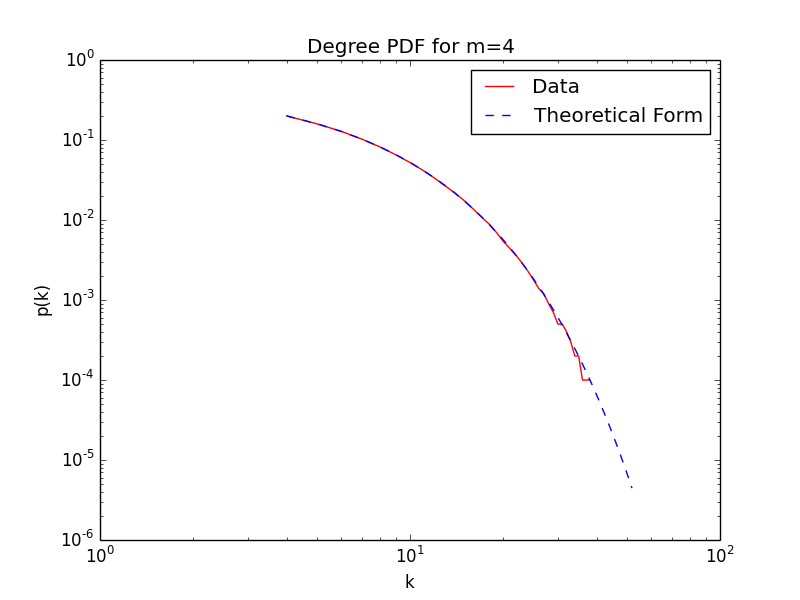
\includegraphics[height=60mm]{comparison22.png}
  \captionof{figure}{Degree distribution for random attachment, with theoretical values also plotted for $m=4$, log-binned to reduce the bad statistics caused by the fat tail.}
\end{center}
\begin{center}
  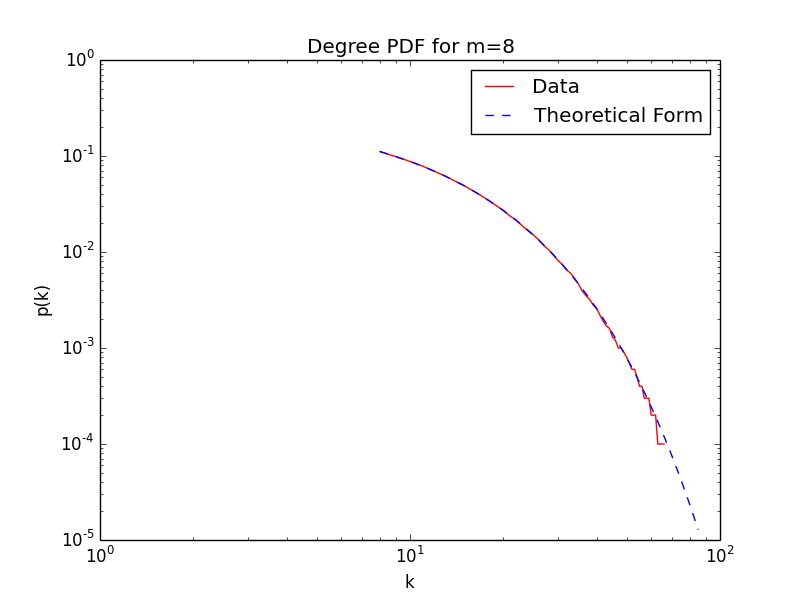
\includegraphics[height=60mm]{comparison32.png}
  \captionof{figure}{Degree distribution for random attachment, with theoretical values also plotted for $m=8$, log-binned to reduce the bad statistics caused by the fat tail.}
\end{center}
\end{multicols}
\begin{center}
    \begin{tabular}{|l|l|l|l|}
    \hline
    $m$ & $\chi^2$ & Degrees of Freedom &p-value \\ \hline
    1 & $1.59266343244 $ & $18$ & 0.999999826223\\ \hline
    2 & $2.30599926631 $ & $29$& 0.999999996191\\ \hline
    4 &  $0.8779577978 $ & $47$&1.0\\ \hline
    8 &  $0.757281441045$ & $77$&1.0\\ \hline
    \end{tabular}
\end{center}
Visually it can be seen from Figures $9-12$ that the simulation behaves exactly as expected. Doing a $\chi^2$-test gives $p-values$ close to 1, beyond any reasonable doubt that the theoretical forms are incorrect, since the p-values are above any of the standard thresholds of significance.

\subsubsection{Largest Degree}
For $N=10000+m$, the predicted values versus the obtained values:

\begin{center}
    \begin{tabular}{|   l|   l|   l|}
    \hline
    $m$ & $\mu(\hat{k}_l)$  & predicted value 	\\ \hline
    1 & $14.11 $&14.29	 		\\ \hline
    2 & $24.51 $ &24.72 			\\ \hline
    4 &  $42.36 $ &45.28			\\ \hline
    8 &  $73.77 $ &86.20			\\ \hline
    \end{tabular}
\end{center}
The first three values match the theory, the last value does not, however the standard deviation increases with $m$, and the larger $m$ was averaged over a number iterations since it takes the longest to run. These values correspond to theory better than the mean average values for the preferential attachment case, because this time the data is not highly skewed, and there is some typical degree that can be defined by the mean. 
\clearpage
\subsection{Random Walks}
\begin{multicols}{2}
\begin{center}
  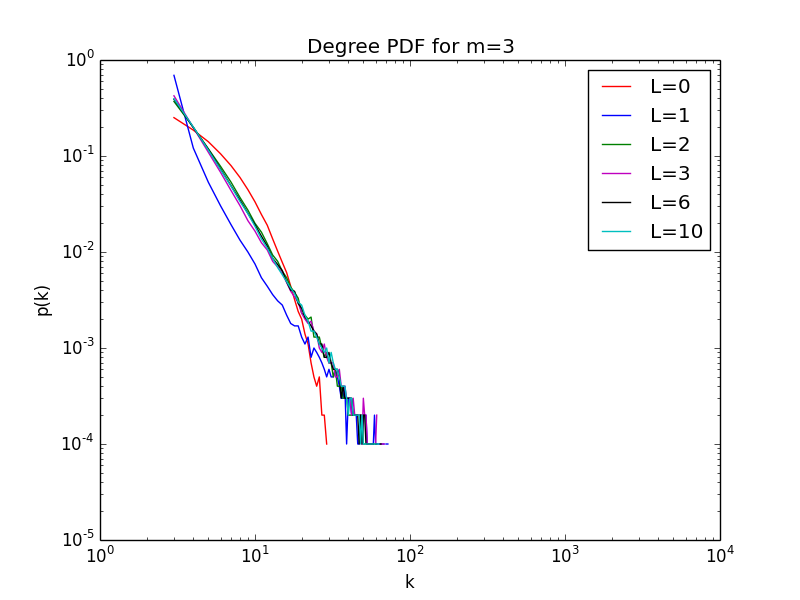
\includegraphics[height=60mm]{degree_dist_RW_unbinned.png}
  \captionof{figure}{Degree distribution for using random walks as the selection method, for different values of $L$}
\end{center}
\begin{center}
  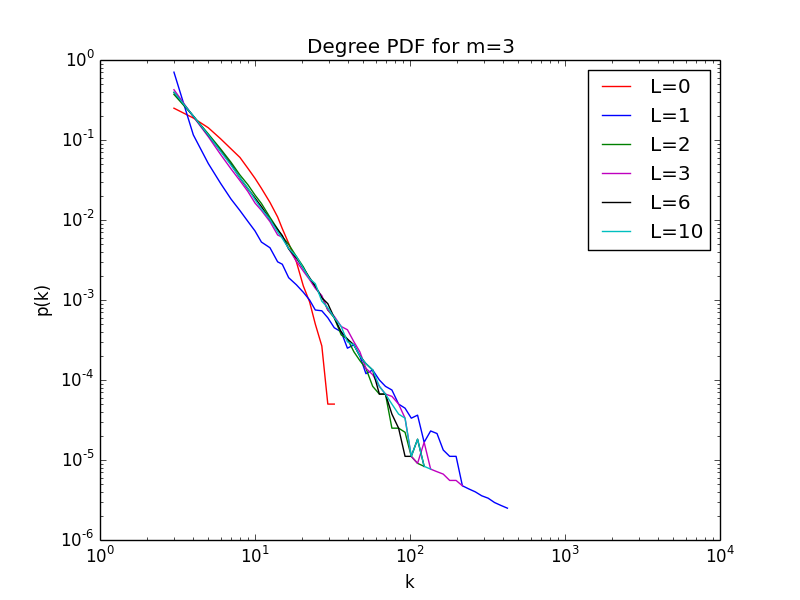
\includegraphics[height=60mm]{degree_dist_RW.png}
  \captionof{figure}{Degree distribution for using random walks as the selection method, for different values of $L$, log-binned to reduce the bad statistics caused by the fat tail.}
\end{center}
\end{multicols}
For the case $L=0$, the degree distribution has an exponential cut off, as opposed to a fat tail. This is expected since the selection is essentially random, so it should look like the random attachment case. For $L=1$, the distribution curves towards the fat-tailed distributions, and appears to be even more skewed and with a higher kurtosis than the fat tailed distributions, this could be because for higher $L$, the random walker can also leave the nodes with high degree, whereas for the $L=1$ case, the random walker only steps towards any node attached to it, which is statistically likely to be a node with high degree. For higher $L$, the distribution is equally fat tailed, suggesting the distribution is of the same form as with preferential attachment, where the node at which the random walker ends up must be proportional to $k$. 

%------------------------------------------------DISCUSSION

\section{Discussion}
The data was sufficient to test the theoretical forms of the distributions. However for comparing the largest degree, it would be useful to compare the predicted values against a larger number of data points. 

None of the results behaved in such a way in which it could not be reconciled with the theoretical predictions of the Barabassi-Albert model or using pure-random attachment.


%------------------------------------------------CONCLUSION

\section{Conclusion}
In conclusion, the Barabassi-Albert model and the pure random attachment model were tested against theoretical forms of the degree distribution, high p-values as a result of the $\chi^2$ test suggests that neither of these contravened the theoretical predictions. the Barabassi-Albert model does indeed give rise to fat tailed distributions for which the degree is scale free. The random-attachment model exponentially cuts off for high degrees. The predicted values of the highest degree matched the observed values , taking the modal average for the Barabassi-Albert model and the mean average for random attachment. 

Data collapse has revealed that there is a finite-size effect that becomes noticeable if the network is growing fast enough. These are values of the degree probability which are higher than predicted in the $t \to \infty$ limit. These are caused by nodes for which there would have been a higher degree if the system size was larger.

Using random walks as the selection for attaching to a new edge, gives rise to fat tailed distributions for the length of the walk greater than 1. For walks of length 0, it is equivalent to random attachment, since the first node of the walk is randomly selected. For walks of length 1, the data shows that the skewness is higher than in the fat-tailed case, this may be because for walks greater than length 1, the random walker also has a chance to leave the first selected node.



%----------------------------------------------------------------------------------------
%	APPENDICES
%----------------------------------------------------------------------------------------
\clearpage 

\section{Appendices}

\subsection{Data Binning}
A probability mass function of the degree $k$ can be estimated by:
\[
P(k) = \lim_{N \to \infty} \frac{N_k}{N}
\]
Where $N_k$ is the frequency in which the degree $k$ occurs. Because $N$ is always finite, there will be clusters of points where $P_{\text{estimated}}=1/N$, this is the minimum that is possible, but the theoretical probability $P(k)$ could have a lower value.

Data binning can be used to map the data onto the actual values. The s-axis is divided into bins, where each bin spans: 
\[
\mathcal{B}_j =[a^j , a^{j+1} [, \;\;\;\;\; j \in \mathbb{Z}^+ \cup \{0\} \quad a>1
\]
If the data $\hat{k} \in \mathcal{B}_j $ occurs, it's recorded as contributing towards the frequency of $ \mathcal{B}_j $. The estimated probabilities are then transformed thusly:
\begin{align*}
\widetilde{P}(k_j) &= \frac{N_j}{N \Delta k} \\
\Delta k & := k_{\text{max}}^j - k_{\text{min}}^j +1 \\
k_j & := \sqrt{k_{\text{max}}^j k_{\text{min}}^j}
\end{align*}
Where $k_{\text{min}}^j$ is the minimum integer value of $\mathcal{B}_j $, $k_{\text{max}}^j$ is the maximum integer value of  $\mathcal{B}_j $. 

In practice $k_{\text{min}}^j$, $k_{\text{max}}^j$ was calculated via:
\begin{align*}
k_{\text{min}}^j & = \floor{a^j} + \delta_{\floor{a^j} \floor{a^{j+1}}} = \left\{ \begin{matrix}\floor{a^j} \quad \floor{a^j} = \floor{a^{j+1}} \\ \ceil{a^j} \quad \floor{a^j} \neq \floor{a^{j+1}}   \end{matrix} \right. \\
k_{\text{max}}^j &= \floor{a^{j+1}} 
\end{align*}
And the bin number to which a data point should belong is calculated as:
\[
j=\floor{\log_a \hat{k}}
\]
Using a dictionary to record the frequencies, the primary keys being the bin numbers. Bins for which there are no integer values (e.g. $[1.1, 1.21 [$) do not exist, in other words they are never included in the data set, otherwise there would be zeros mixed in with the higher values. This has the effect of the apparent loss of detail for low values of $s_j$ and causes the oscillations near the beginning of the plots in the graphs.






%----------------------------------------------------------------------------------------
%	REFERENCE LIST
%----------------------------------------------------------------------------------------
\clearpage
\begin{thebibliography}{99} % Bibliography - this is intentionally simple in this template

\bibitem[1]{cc}
\newblock Evans, Tim. 
\emph{lecture Notes, Networks}

\bibitem[2]{script}
\newblock Evans, Tim, Christensen, Kim 
\emph{Complexity and Networks Project Notes}

\newblock
Imperial College London 2014
 
\end{thebibliography}

%----------------------------------------------------------------------------------------



\end{document}
